
The electrical model consists of low-voltage (LV) and high-voltage (HV) circuits, depicted in
Fig.~\ref{electrical_model}. The LV current is used to power the hybrid controller chips (HCCs),
ATLAS Binary Chips (ABCs) and Autonomous Monitoring and Control chip (AMAC) located on PCBs that are
glued directly onto the surface of the sensor. The number of chips vary according to the design of
each different module type (barrel short-strip and long-strip modules, and six different endcap
module designs).

\begin{figure}[ht!]
\centering
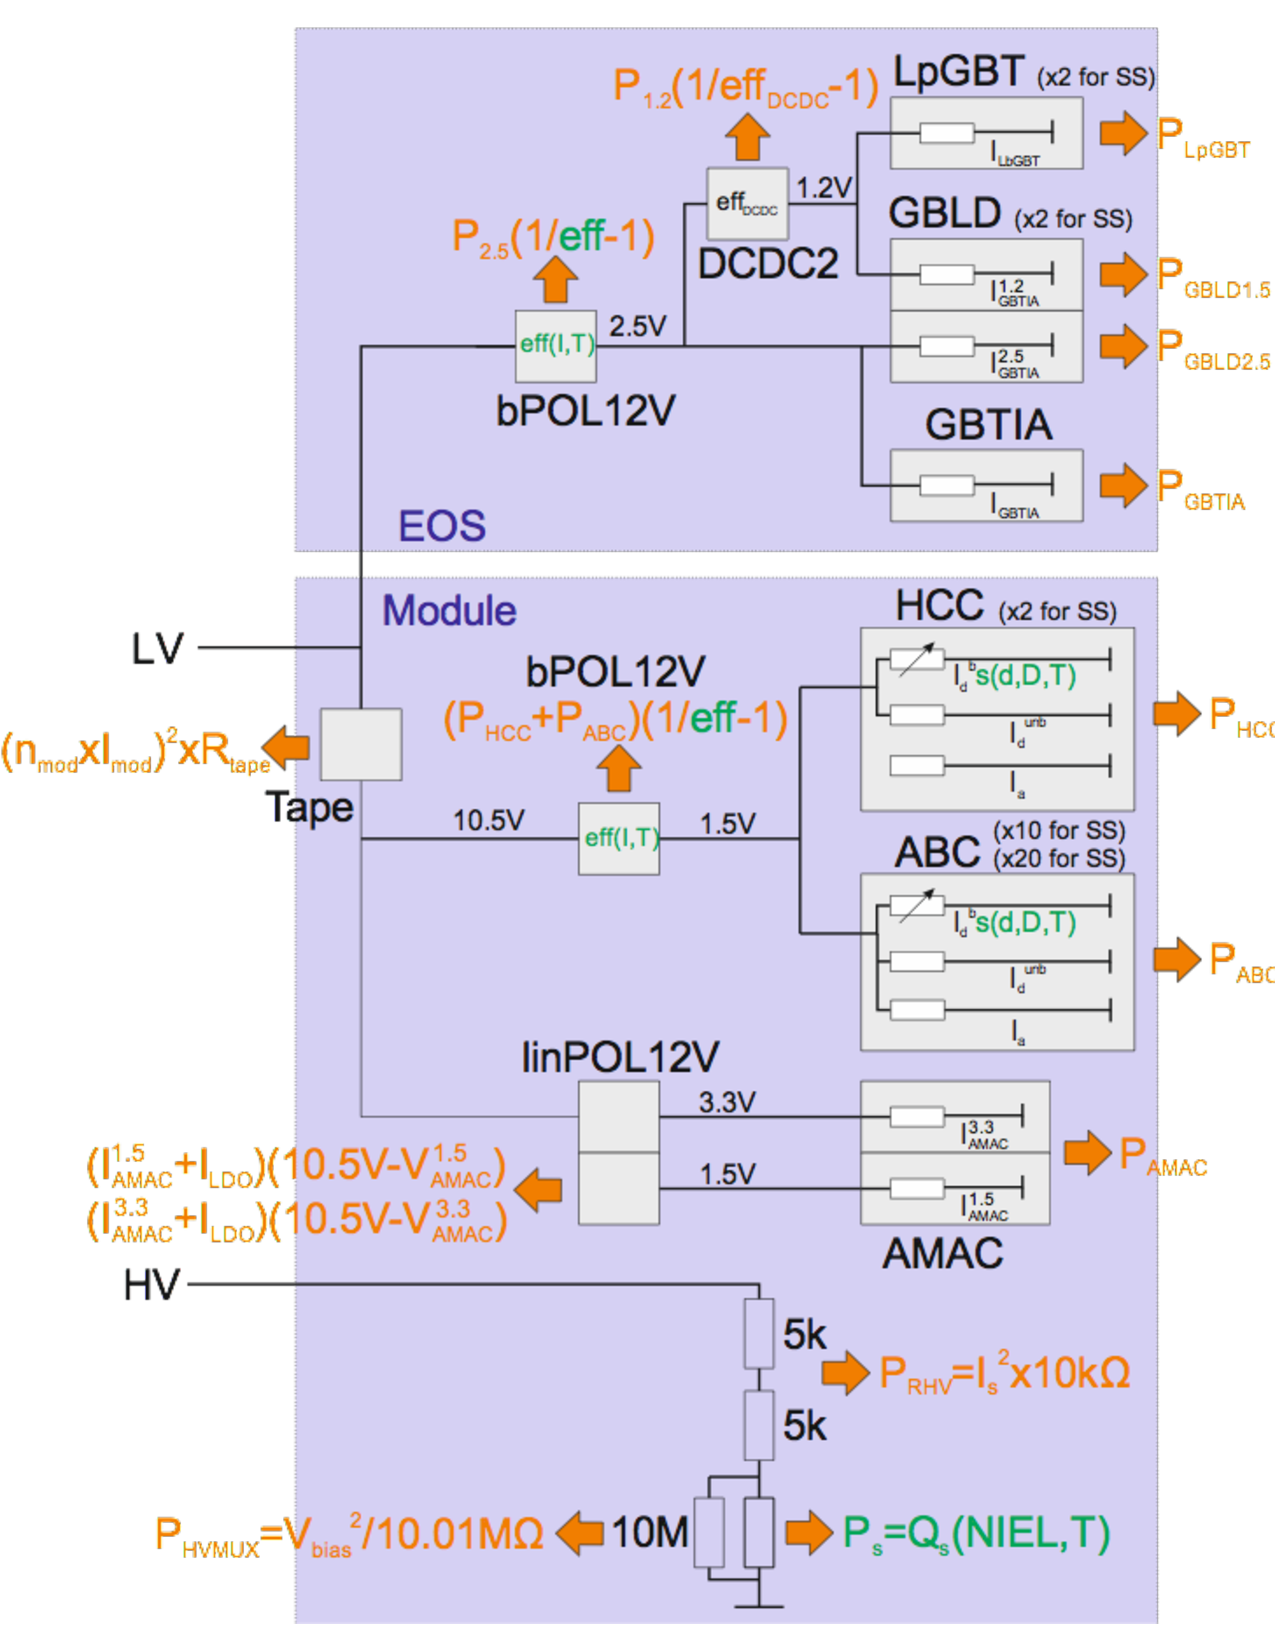
\includegraphics[width=0.8\linewidth]{figures/electrical_model.pdf}
\caption{
The electrical model of the ITk Strip barrel and endcap modules.
}
\label{electrical_model}
\end{figure}

The ABCs and HCCs are all powered at 1.5~V using a DCDC converter (the FEAST) to step the voltage down
from 11~V. Typically one FEAST per module is used to power the chips; however, due to the large
number of ABCs on endcap module R3, the load is split across two FEAST converters on the module.

The AMAC contains a component powered at 1.5~V and one powered at 3~V; both are delivered from the
11V source by an LDO regulator with a 1.9~mA quiescent current.
Again, the endcap module R3 differs from other modules, containing two AMACs each powered by its own
LDO.

The bus tape, which carries both LV and HV currents, has a small wire resistance, which impacts the
module in two ways. First,
the tape itself will radiate some heat according to the amount of current passing through it; this
source of heat is accounted for in the model, however the contribution to the total module power
is negligible.
Second,
the voltage supplied to the module will be affected by the small $\Delta V$ in the bus tape. This
effect is largest for modules on the non-EOS end of the barrel stave or endcap petal, where the current
has traveled a longer distance. The treatment of this effect is slightly different in the barrel and
endcap models: in the barrel, the voltage delivered to every module is set at 10.5~V; in the endcap,
the $\Delta V$ is estimated based on the calculated expected power loss along the tape for each module.
In both cases, the impact of using a different treatment is small.

The low-voltage current is also delivered to the EOS card to power various data transfer components,
which require 2.5~V and 1.2~V currents.
On the EOS, a FEAST identical to the one used on the module is used to step the voltage down from 11~V
to 2.5~V; an additional LDO regulator brings  2.5~V down to 1.2~V for some components.
The EOS cards on the endcap petals and the long-strip staves have one GBLD and one LpGBT;
EOS cards on the short-strip staves contain two of each. All EOS cards contain one GBTIA.

Finally, the HV current provides the voltage bias on the silicon sensors. An HV multiplexer
switch (HVMUX) is placed in parallel to the sensor, which can be used to disconnect the sensor from the
bias line. Two HV filters with an effective resistance of 10~k$\Omega$ are placed in series with the
sensor. The nominal operating voltage of the sensor is expected to be 500V, but the system is designed
to operate with a voltage bias of up to 700V.
